\section{Mirabilandia today}\label{sec:mirabilandia-today}
The amusement park to date offers limited technological support to visitors.
As a result, all activities are carried out in a ``traditional'' manner:
for instance, there is no technological support for queue management, they only provide the
``Flash Pass''\footnote{\url{https://www.mirabilandia.it/en/organizza-la-tua-visita/attivita/flash-pass}} (a paper card or bracelet that gives you
priority access to the attractions by a reserved entrance) that has no virtual queueing system integration.

In addition, there is no system to improve the visitor experience based on either the visitor's preferences or external factors that may affect the
quality of their visit.

However, some technological aspects can be found in the park:
there are some ``totems'' placed around that give information about the attractions and the current waiting time, but they are not connected with sensors or other smart devices.
We have no information on how the waiting time is calculated and, based on empiric considerations, it turns out to be approximate and not very indicative of reality.
In figure~\ref{fig:mira-totem} there is an example of a totem placed in the park.

\begin{figure}[H]
	\centering
	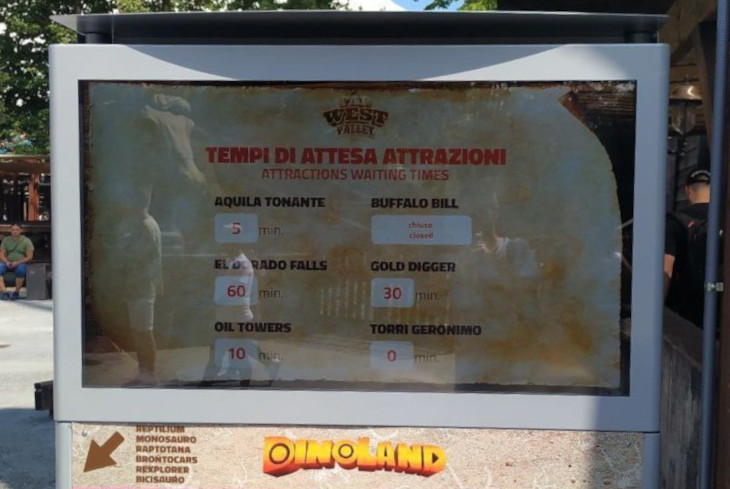
\includegraphics[width=0.8\textwidth]{img/mira-totem.jpg}
	\caption{A totem showing the average waiting time for each attraction in the Mirabilandia park.}
	\label{fig:mira-totem}
\end{figure}

Mirabilandia provides a very simple app\footnote{\url{https://www.mirabilandia.it/en/prima-del-tuo-arrivo/la-nostra-app}} for smartphones that, however, doesn't have the characteristics needed for a proper Micro City experience.
In fact, only allows the \textit{visitors} to:
\begin{itemize}
	\item buy tickets
	\item consult an interactive map
	\item visualize pre-defined and static itineraries
	\item consult shows' beginning time
	\item select a pre-defined and static plan by attraction's category: ``extreme'', ``for families'', ``wet'', ``for families'' and ``for children'' (Figure\ref{fig:miraApp})
\end{itemize}

Lastly, Mirabilandia offers a very simple virtual queueing service Qoda\footnote{\url{https://get.qoda.app/}} for three refreshment points and stores\footnote{\url{https://www.mirabilandia.it/mir-blog-export/qoda-la-tua-fila-virtuale}}.
It works by scanning a QR code one can find at the point of interest and it will immediately tell the waiting number on the person's mobile phone, as well as the estimated time for their turn.
This time is however based on the number of people that scanned the QR code and doesn't consider any other factor.

\begin{figure}[H]
	\centering
	\begin{subfigure}[b]{0.35\textwidth}
		\centering
		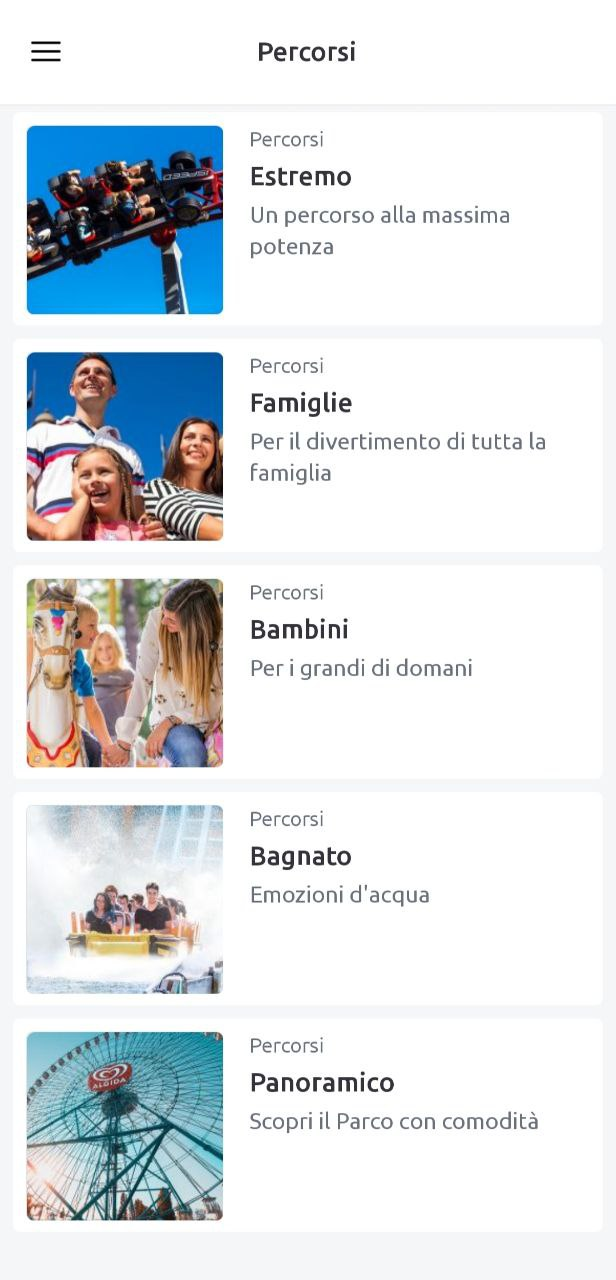
\includegraphics[width=\textwidth]{img/miraPlan}
	\end{subfigure}
	\begin{subfigure}[b]{0.35\textwidth}
		\centering
		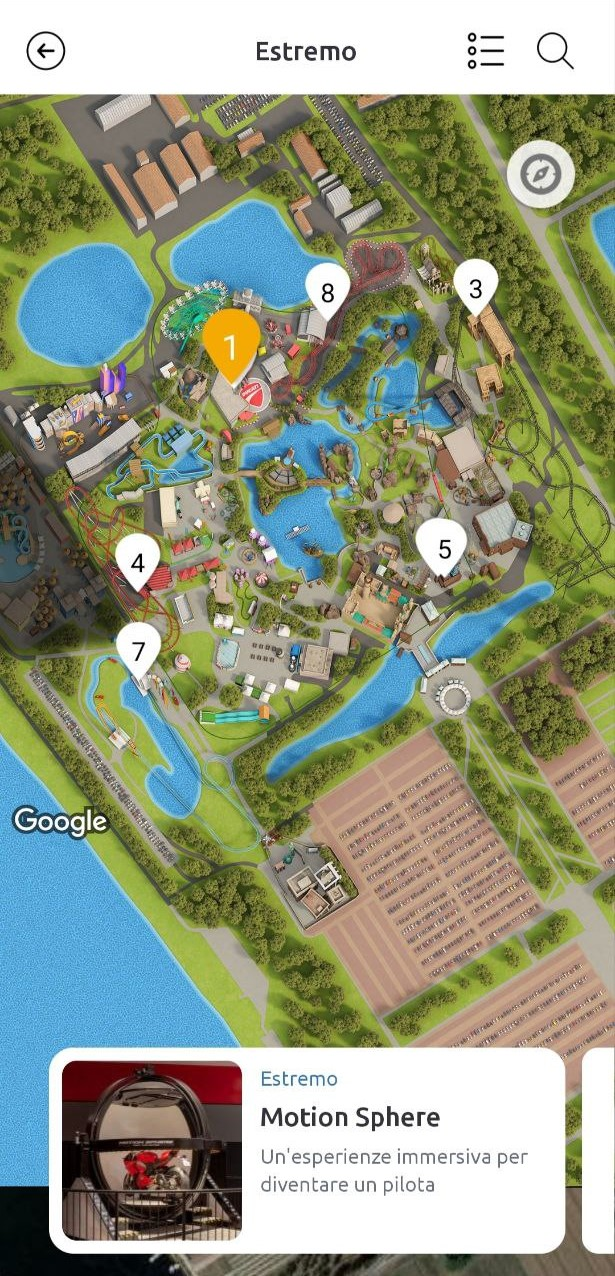
\includegraphics[width=\textwidth]{img/miraextr}
	\end{subfigure}
	\caption{Mirabilandia App's planning a visit screenshots}
	\label{fig:miraApp}
\end{figure}

% Queues at the various attractions are still conducted traditionally, without any technological support.
% At present, Mirabilandia amusement park does not have a queue management system or a recommendation system for its guests.
% The amusement park only provides totems that indicate an average wait time for each attraction.
% However, the stated time turns out to be very often approximate and not very indicative of reality.
% In recent years, the ``flash pass'', a facility that allows guest to skip the line, has been introduced.
% Again, such a system has no technological support: guests must go to the ride in advance and indicate the time they intend to participate.

% Mirabilandia does not currently provide any recommendation system: all activities within the park are independent and do not actively collaborate
% with it to incentivize guests to interact with these activities.

\section{Currently available services and technologies for smart amusement parks}\label{sec:state-of-the-art-analysis}
This section will discuss the state of the art of technologies already used in amusement parks around the world.
The main purpose is to understand what would be the best ``smart'' and innovative technological options to use in Mirabilandia nowadays considering the Micro City context.
As seen in the documents ``Micro City - Domain Analysis'' and ``Micro City - Case Study Analysis'', an Amusement Park as a Micro City has the following necessities:
\begin{itemize}
	\item Queue management: the park may want to offer its visitors the possibility of reducing the waiting time to access an attraction, event or a food service
	\item Personalization of the experience: recommendation systems may be used by the park to suggest attractions, restaurants, events, etc.
	      based on the visitors' interests
	\item Proximity/localization suggestions: visitors may receive on their wearable device some notifications concerning marketing, offers or the queue with fewer wait-time based on their position within the park
\end{itemize}

There are many solutions adopted by some amusement parks to support the previous points.
For instance, the avoiding long lines problem is faced with virtual queueing\footnote{\url{https://en.wikipedia.org/wiki/Virtual_queue}} systems
and for recommendation and proximity marketing\footnote{\url{https://en.wikipedia.org/wiki/Proximity_marketing}} there are many different solutions.

The following sections are intended to provide an overview of companies' products and technologies already used in amusement parks around the world.

\subsection{Accesso Technology Group}\label{subsec:accesso-technology-group}
Accesso Technology Group\footnote{\url{https://www.accesso.com/}} (formerly Lo-Q) is an English company that provides different solutions
mostly to amusement parks like the ``Six Flags'' corporation in the US and ``LEGOLAND Windsor Resort'' in the UK but also to airports,
ski facilities, events and places that need social distancing management and so on.
Their two main solutions of interest for a Micro City context are a virtual queueing system and the personalization of
the guests' experience by sending them tailored content, offers and recommendations.
Furthermore, along with their virtual queueing products they integrate a location-based messaging system.

\subsubsection{Lo-Queue Virtual Queueing Products}
Their patented~\cite{q-management-system-patent} \cite{q-system-patent}
virtual queueing technology allows a virtual queue to dynamically adjusts to many different unpredictable real-time variables such
as guest flow, bad weather, ride down time, etc.
automatically revising waiting times and communicating real-time updates to guests.
The mechanism, simply lets the guests choose a ride and, when their turn comes, are notified to head to the attraction.

Their two current products for virtual queueing are \textit{Qsmart} and \textit{Prism}\footnote{\url{https://www.accesso.com/solutions/virtual-queuing/prism}}.
The former allows people to access the virtual queueing services directly from their smartphones, whereas the latter is a ``smartwatch-like''
wearable.

In 2009, Mirabilandia used to sell to its guests the Accesso's \textit{Qbot} device -- a previous version of Prism -- named ``V-Pass''\cite{v-pass-mira}, but is no
longer available to this days.

\subsubsection*{Prism}
Prism is a standalone device, with no need for kiosks or charging stations to support its use.
Moreover, it is waterproof, hypoallergenic and durable~\cite{prism-desc}.
As can be observed in Figure~\ref{fig:prism}, Prism provides the following functionalities:
\begin{itemize}
	\item Virtual queueing: guests can manage their reservation in line and monitor the line status
	\item Payments: guests can make payments via secure NFC technology
	\item Messaging: guests can receive push notifications for proximity-based marketing (i.e.\ trigger nearby events based on people location, Figure~\ref{fig:prism-icecream}), operational updates, or the status of pending virtual queue positions
	\item Photography: Prism allows automated tagging of ride and park photographs
	\item Access: guests can easily access park turnstiles, guest lockers, resort hotel rooms, etc.
	\item Intelligence: Prism collects real-time information about the users' behaviour during the visit for marketing and park operations purposes
\end{itemize}

\begin{figure}[H]
	\centering
	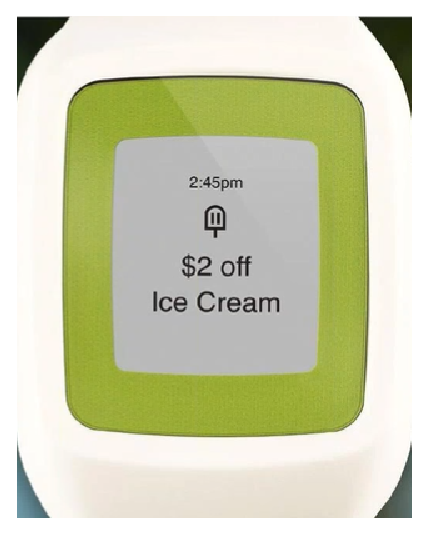
\includegraphics[width=0.3\textwidth]{img/prism-icecream}
	\caption{Example of a push notification based on the visitor proximity to an ice cream shop}
	\label{fig:prism-icecream}
\end{figure}

Prism works on a \textbf{proprietary network} and uses three ways to communicate:
\begin{itemize}
	\item \textbf{Bluetooth Low Energy:} allows \textit{visitors} to receive real-time messages based on their location, and the park gains valuable insights about visitors' flow throughout the park
	\item \textbf{Near Field Communication (NFC):} used for access, payments, rentals, etc.
	\item \textbf{Long Range Sub-GHz Two-Way Radio:} allows \textit{visitors} to reserve and modify queueing reservations from where they are without having to use their smartphone
\end{itemize}

The wearable is made with waterproof materials and carries a vibrator motor for haptic feedback to interact with the user and send alerts.
Moreover, its battery supports over 200 days of usage.
Technical specifications~\cite{prism-manual} are listed in Tables~\ref{tab:ci-tec-spec},~\ref{tab:pr-tec-spec},~\ref{tab:c-tec-spec}.

\begin{table}[H]
	\centering
	\begin{subtable}[t]{0.85\textwidth}
		\centering
		\begin{tabular}{|l|l|}
			\hline
			LCD            & LCD Display, 3 bit colour, Resolution 176 x 176 \\ \hline
			Vibrator motor & 1,000 rpm                                       \\
			\hline
		\end{tabular}
		\caption{Controls and Indicators}
		\label{tab:ci-tec-spec}
	\end{subtable}
	\begin{subtable}[t]{0.85\textwidth}
		\centering
		\begin{tabular}{|l|l|}
			\hline
			Battery      & CR3032 Lithium Ion coin cell \\ \hline
			Average life & 200 days or 2,000 hours      \\
			\hline
		\end{tabular}
		\caption{Power Requirements}
		\label{tab:pr-tec-spec}
	\end{subtable}
	\begin{subtable}[t]{0.85\textwidth}
		\centering
		\begin{tabular}{|l|l|}
			\hline
			Long Range   & 868MHz \& 915MHz (SubGHz) transceiver \\ \hline
			Medium Range & 2.4GHz BLE transceiver                \\ \hline
			Short Range  & Secure 14443 RFID/NFC device          \\
			\hline
		\end{tabular}
		\caption{Communications}
		\label{tab:c-tec-spec}
	\end{subtable}
	\caption{Prism technical specifications}
	\label{tab:prism-tech-spec}
\end{table}

\subsubsection*{QSmart}
On the other hand, QSmart is a ready-to-use platform and utilizes the guest's smartphone hardware, is cloud based
and operates via Wi-Fi.

In addition to the features already listed for Prism, Qsmart gives the possibility to:

\begin{itemize}
	\item easily make rides and
	show ticket purchases with a mobile payments system which is
	PCI\footnote{\url{https://en.wikipedia.org/wiki/Payment_Card_Industry_Data_Security_Standard}} compliant
	\item allows choosing among a different set of ride packages with different perks depending on the price
	\item validate the ride by a ride attendant who scans a QR code on the guest's smartphone
	\item can be integrated with other Accesso products like, for instance, an online ticketing system.
	
\end{itemize}

\begin{figure}[H]
	\centering
	\begin{subfigure}[b]{0.85\textwidth}
		\centering
		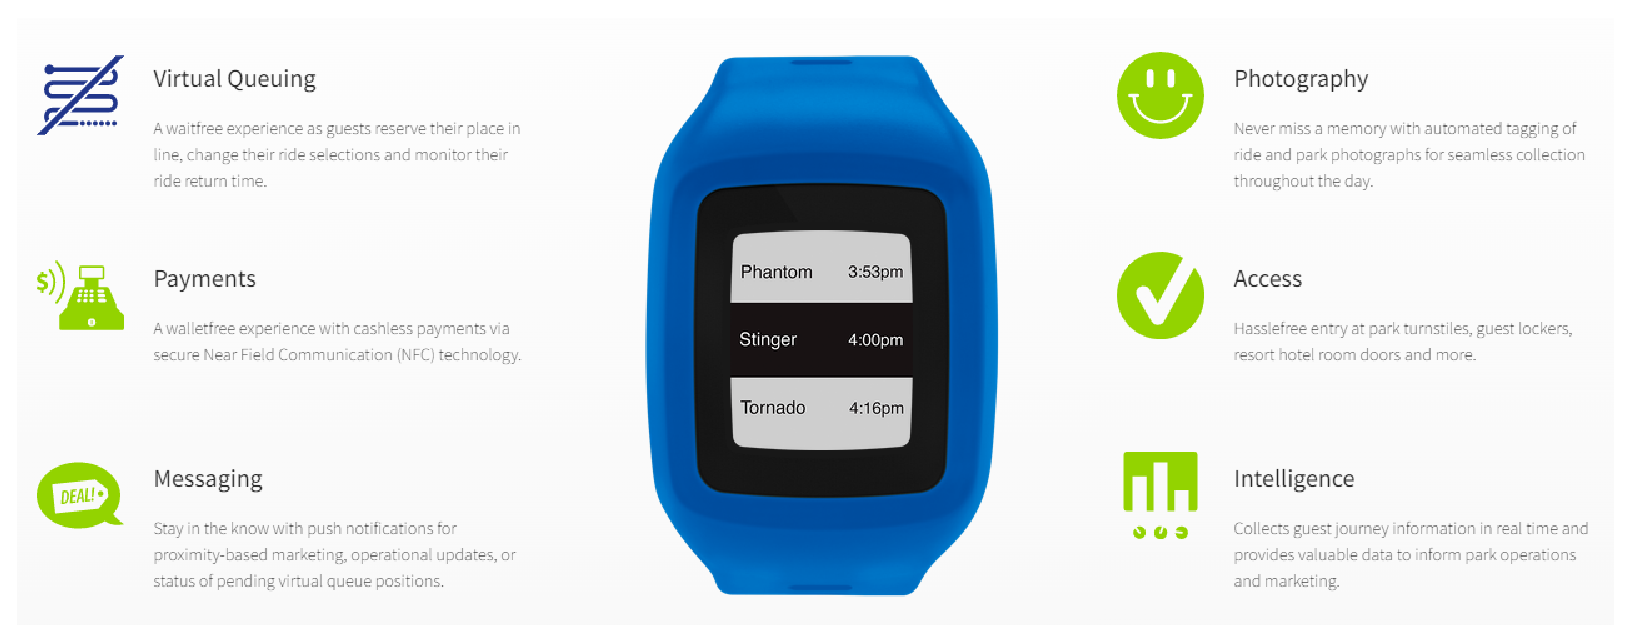
\includegraphics[width=\textwidth]{img/prism}
		\caption{Prism main functionalities}
		\label{fig:prism}
	\end{subfigure}
	\hfill
	\begin{subfigure}[b]{0.85\textwidth}
		\centering
		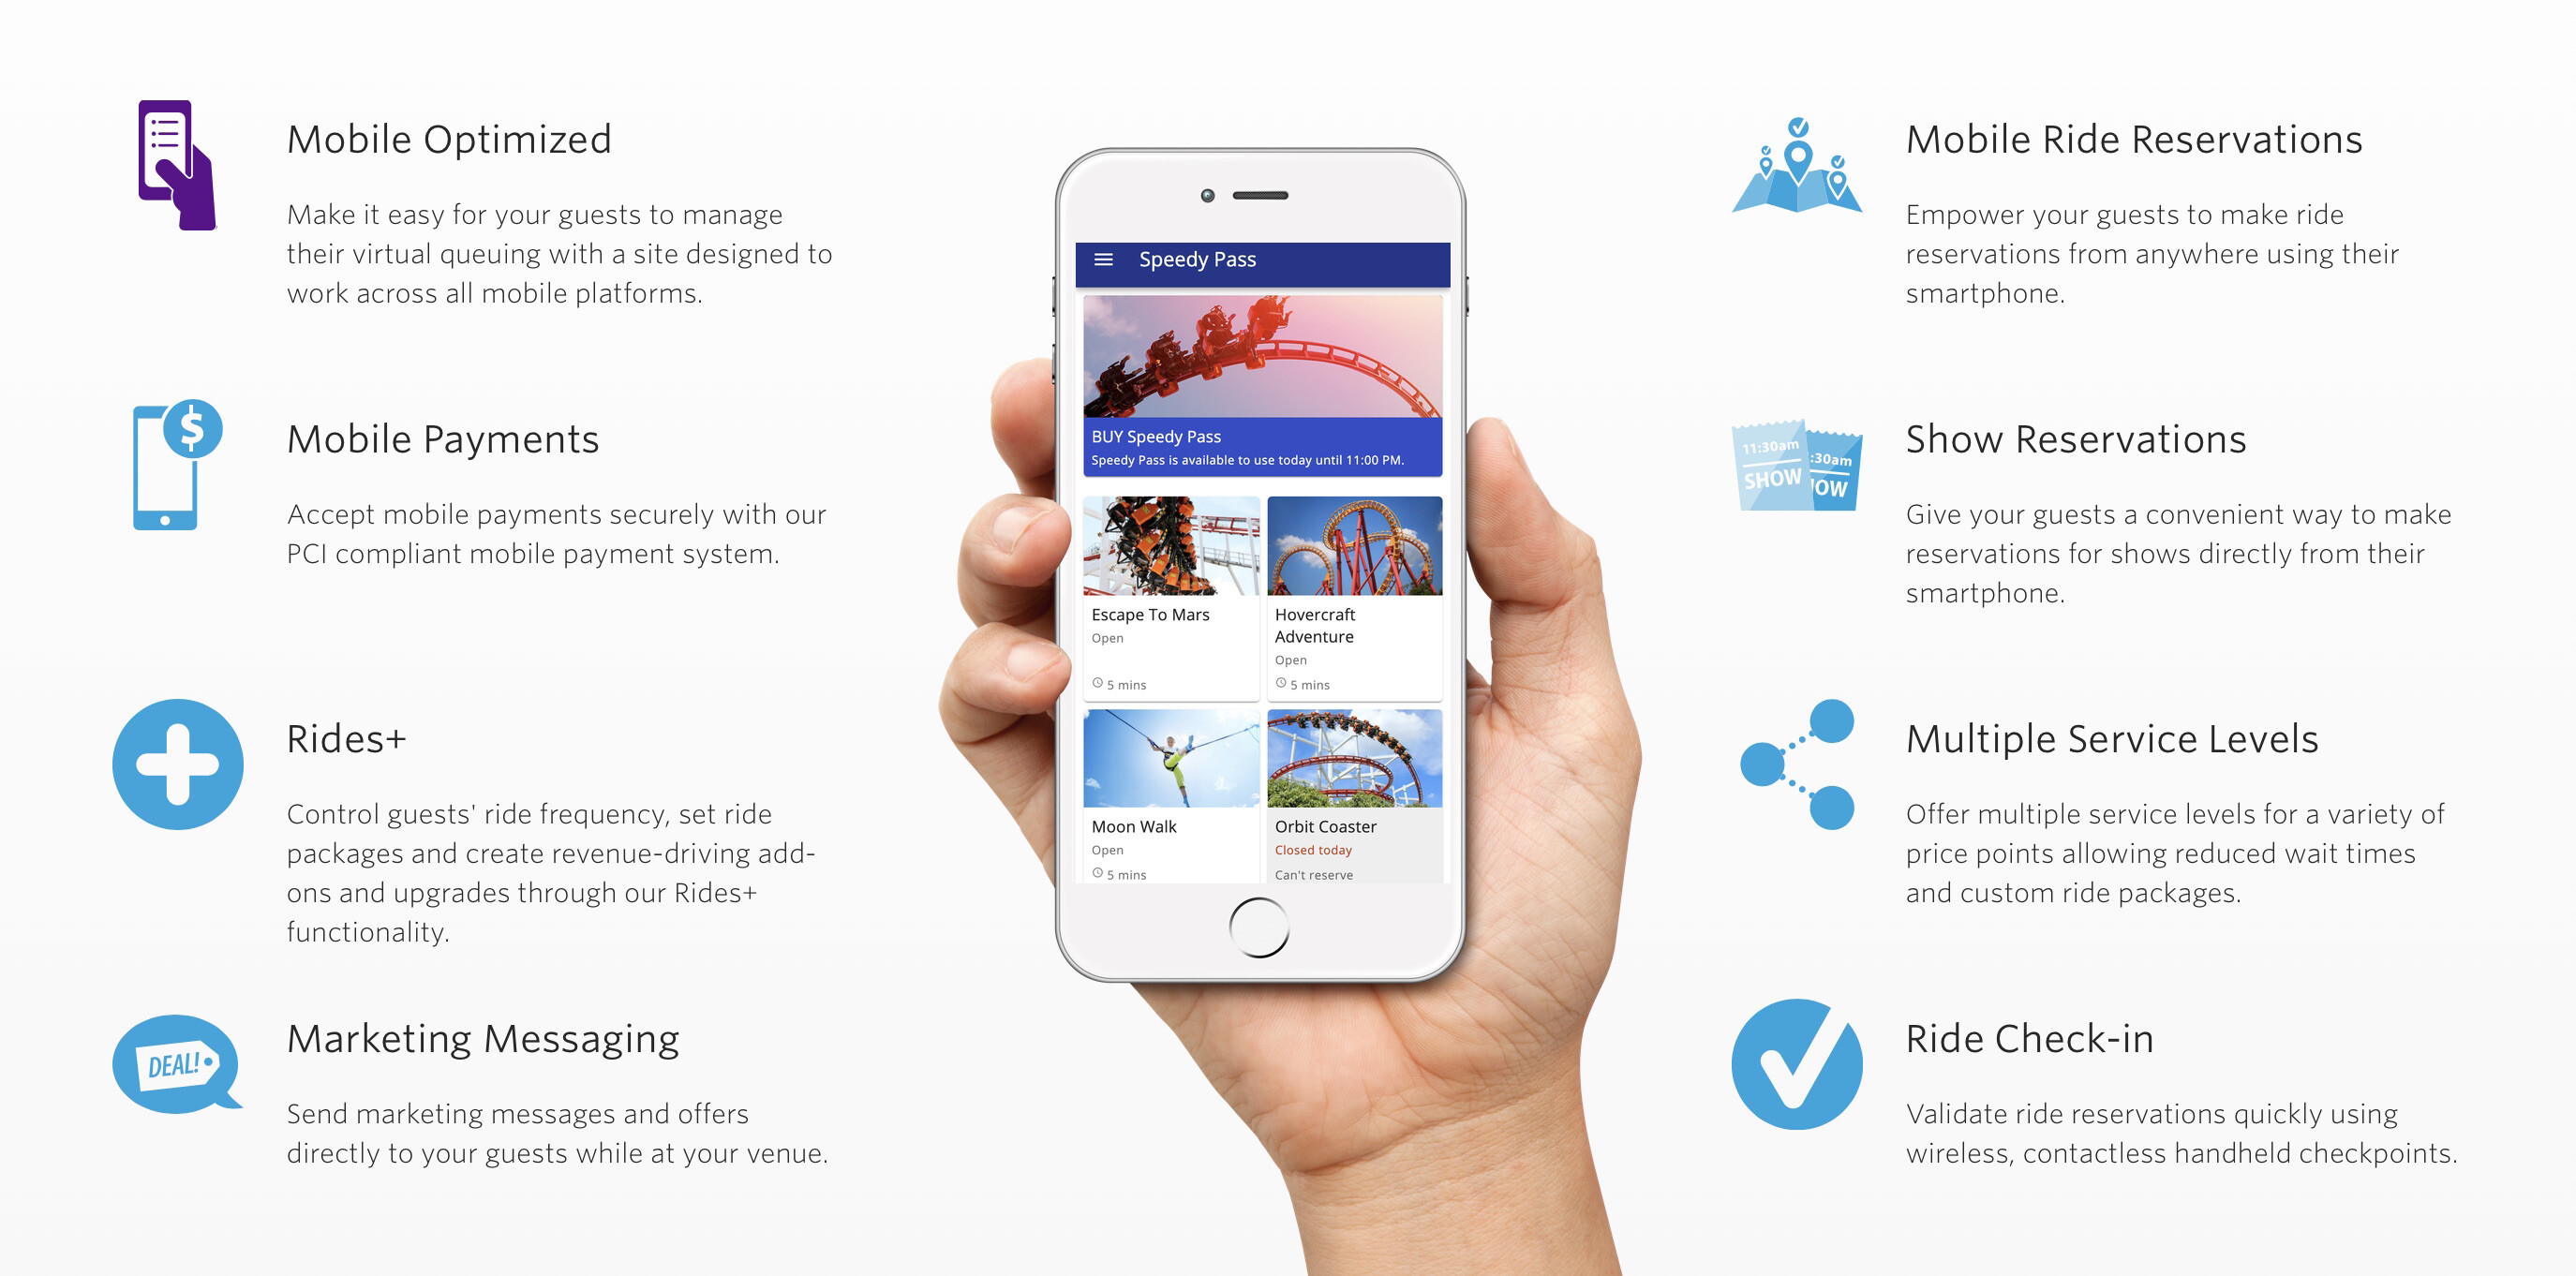
\includegraphics[width=\textwidth]{img/qsmart}
		\caption{Qsmart main functionalities}
		\label{fig:qsmart}
	\end{subfigure}
	\caption{Accesso's products for virtual queueing\protect\footnotemark}
	\label{fig:prismart}
\end{figure}
\footnotetext{\url{https://www.accesso.com/solutions/virtual-queuing}}

Both Prism and QSmart interact with the Virtual Queue Management System, where customers can consult
analytics and performance data as well as centralized data on park attendance.
It is also possible to check ride usage, guests activity, ride downtime and transactional data per user and how long they waited for each ride.

Finally, it is possible to control in real-time the virtual queueing solution.

\subsubsection{The Experience Engine (TE2) Recommendation system}
The Experience Engine\footnote{\url{https://www.accesso.com/solutions/guest-experience}} is a platform-as-a-service (PaaS) technology
which allows the park to connect with guests in real-time and provides them with relevant offers, messages and recommendations.
It is integrated with Accesso's Virtual Queueing Products and could work as a location-based targeted system~\cite{accesso-location-based-exp} helping alleviate
long lines by driving traffic to other less utilized outlets, or by incentivizing guests to dine before or after the rush
hours with special offers.
The platform communicates with Bluetooth Beacons\footnote{\url{https://en.wikipedia.org/wiki/Bluetooth_low_energy_beacon}} and,
whenever a guest's device receives a beacon signal, the device notifies the TE2 platform of the proximity to a beacon.
TE2 then determines the visitor's real interest in a scheduled experience.
If so, the visitor will receive a notification.
Thanks to this platform, Accesso's clients can create custom itineraries for every park's visitor.
In Figure~\ref{fig:te2ex} is synthesized the TE2 functioning.

\begin{figure}[H]
	\centering
	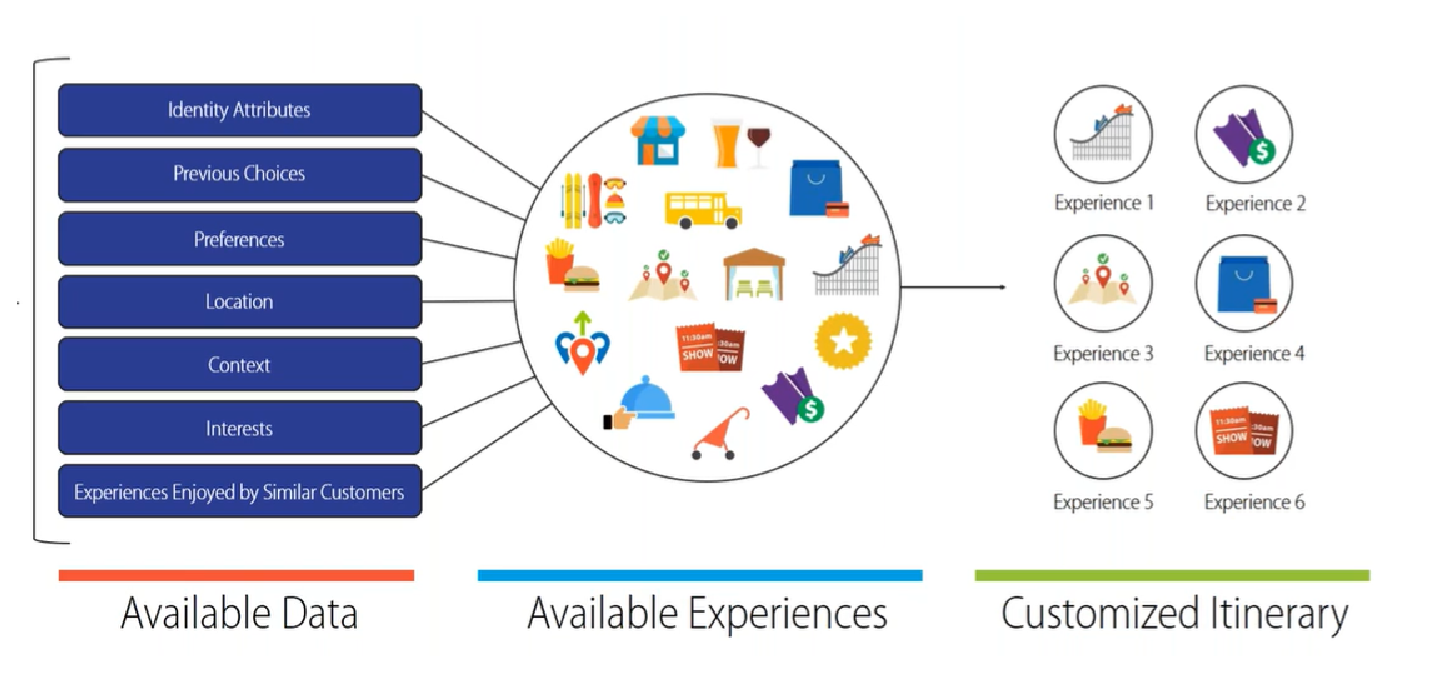
\includegraphics[width=0.9\textwidth]{img/te2ex}
	\caption{TE2 functioning}
	\label{fig:te2ex}
\end{figure}

\subsection{Disney Parks, Experiences and Products}\label{subsec:disney-parks-experiences-and-products}
Disney Parks, Experiences and Products, Inc., is one of The Walt Disney Company's business.
In its parks ``Walt Disney World'', Florida and ``Disneyland Resort'', California offers their guests solutions
for virtual queuing and a recommendation.
In fact, guests can use the ``My Disney Experience'' app and enjoy the ``Disney Genie'', ``Disney Genie+'' and ``Lighting Lane''\footnote{\url{https://www.disneyworld.eu/genie/information/}} services.
The former is free of charge whether ``Genie+'' and ``Lighting Lane'' have additional costs.
The perks in Figure\ref{fig:dgenie} are the following:

\begin{itemize}
	\item Tailored recommendations: guests can receive attraction and dining recommendations based on what is the preferred visiting plan they previously told
	      to the service
	\item Virtual assistant: provides a virtual assistant to ask questions about the park
	\item Time-based suggestions: it displays a good time to go to a suggested experience and an idea of the forecasted wait for attractions, entertainment and dining
	\item Booking activities: order food, make dining reservations, check into a restaurant, request to join an available virtual queue or book arrival times in a reserved entrance for
	      some activities.
\end{itemize}

\begin{figure}[H]
	\centering
	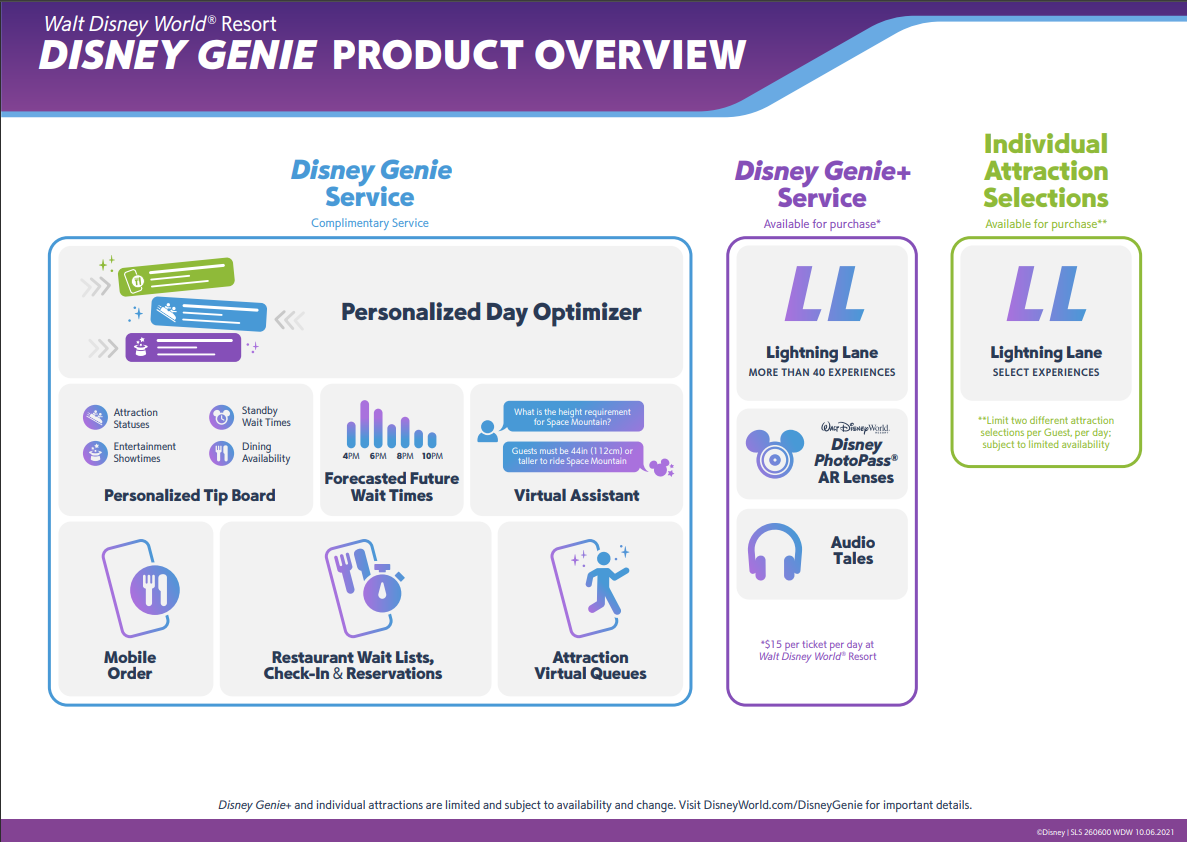
\includegraphics[width=0.8\textwidth]{img/dgenie}
	\caption{Disney Genie services}
	\label{fig:dgenie}
\end{figure}
